% ============================================================
%  1D Thermal Diffusion — Fundamentals and Discretisation
%  C. Shannon — March 2026
% ============================================================
\documentclass[11pt, a4paper]{scrartcl}

% --- Packages ---
\usepackage[british,UKenglish,USenglish,english,american]{babel}
\usepackage[tmargin=1in, bmargin=1in, lmargin=0.75in, rmargin=0.75in]{geometry}
\usepackage{amsmath, amssymb}
\usepackage{physics}          % \dv, \pdv, etc.
\usepackage{siunitx}
\usepackage{booktabs}
\usepackage{array}
\usepackage{geometry}
\usepackage{mathtools}
\usepackage{xcolor}
\usepackage{listings}
\usepackage{caption}
\usepackage{hyperref}
\usepackage{tikz}
\usepackage{setspace}
\usetikzlibrary{arrows.meta, decorations.markings, patterns}

\geometry{margin=2.5cm}

\sisetup{
  output-decimal-marker = {.},
  per-mode = symbol
}

% Colours
\definecolor{myblue}{RGB}{30, 90, 180}
\definecolor{myred}{RGB}{180, 30, 30}
\definecolor{mygray}{RGB}{240, 240, 240}
\definecolor{codegreen}{RGB}{0,128,0}
\definecolor{codegray}{RGB}{128,128,128}

% MATLAB listing style
\lstdefinestyle{matlab}{
  language=Matlab,
  basicstyle=\ttfamily\small,
  keywordstyle=\color{myblue}\bfseries,
  commentstyle=\color{codegreen}\itshape,
  stringstyle=\color{myred},
  backgroundcolor=\color{mygray},
  frame=single,
  rulecolor=\color{gray!50},
  numbers=left,
  numberstyle=\tiny\color{codegray},
  numbersep=8pt,
  breaklines=true,
  captionpos=b
}

% Hyperref
\hypersetup{
  colorlinks=true,
  linkcolor=myblue,
  urlcolor=myblue
}

% ============================================================
\begin{document}

\begin{center}
  {\LARGE\bfseries\color{myblue} 1D Thermal Diffusion}\\[6pt]
  {\large Physical Fundamentals, Discretisation, and MATLAB Implementation}\\[8pt]
  {\normalsize C. E. Shannon \quad|\quad March 2026}
\end{center}

\vspace{0.5em}
\hrule height 1.2pt
\vspace{1.5em}

\tableofcontents

\vspace{1.5em}
\hrule
\newpage
\begin{onehalfspace}
% ============================================================
\section{Problem Geometry and Parameters}

An aluminium bar with the following geometric and thermophysical properties is considered:

\begin{table}[h!]
\centering
\caption{Physical parameters of the problem}
\begin{tabular}{llll}
\toprule
\textbf{Quantity} & \textbf{Symbol} & \textbf{Value} & \textbf{Unit} \\
\midrule
Length                        & $L$             & \num{50}            & \si{\milli\meter} \\
Cross-sectional area          & $A$             & $\num{3} \times \num{30}$ & \si{\milli\meter\squared} \\
Thermal diffusivity (Al)      & $\alpha$        & \num{98e-6}         & \si{\meter\squared\per\second} \\
Thermal conductivity (Al)     & $k$             & \num{237}           & \si{\watt\per\meter\per\kelvin} \\
Applied power at $x=0$        & $q_\text{in}$   & \num{25}            & \si{\watt} \\
Heat-sink temperature at $x=L$& $T_\text{sink}$ & \num{80}            & \si{\celsius} \\
Initial temperature           & $T_0$           & \num{80}            & \si{\celsius} \\
\bottomrule
\end{tabular}
\end{table}

The spatial domain is $x \in [0,\, L]$. The boundary conditions are:
\begin{itemize}
  \item \textbf{Left boundary} ($x = 0$): prescribed heat flux \textbf{(Neumann)};
  \item \textbf{Right boundary} ($x = L$): fixed temperature \textbf{(Dirichlet)}.
\end{itemize}

\begin{figure}[h!]
\centering
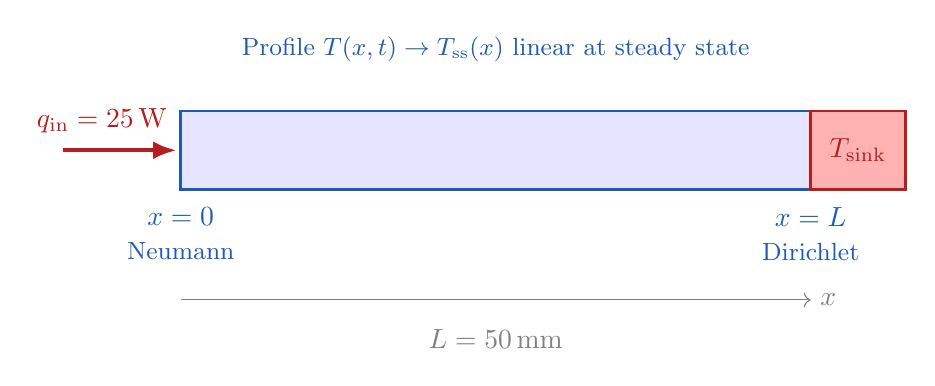
\begin{tikzpicture}[scale=1.0]
  % Bar
  \fill[blue!10, draw=myblue, line width=1pt] (0,0) rectangle (8,1);
  % Incoming flux arrow
  \draw[-{Latex[length=3mm]}, myred, line width=1.5pt] (-1.5, 0.5) -- (-0.05, 0.5);
  \node[myred, above] at (-1, 0.6) {$q_\text{in} = \SI{25}{\watt}$};
  % Left boundary label
  \node[myblue, below] at (0, -0.1) {$x=0$};
  \node[myblue, below] at (0, -0.55) {\small Neumann};
  % Right heat sink
  \fill[red!30, draw=myred, line width=1pt] (8,0) rectangle (9.2,1);
  \node[myred] at (8.6, 0.5) {$T_\text{sink}$};
  \node[myblue, below] at (8, -0.1) {$x=L$};
  \node[myblue, below] at (8, -0.55) {\small Dirichlet};
  % x-axis
  \draw[->, gray] (0,-1.4) -- (8,-1.4) node[right] {$x$};
  \node[gray, below] at (4,-1.65) {$L = \SI{50}{\milli\meter}$};
  % Temperature profile arrow
%  \draw[->, dashed, myblue, line width=1pt] (0.3, 1.3) to[out=0, in=170] (7.7, 0.9);
  \node[myblue, above] at (4, 1.5) {\small Profile $T(x,t) \to T_\text{ss}(x)$ linear at steady state};
\end{tikzpicture}
\caption{Domain schematic: bar with prescribed flux on the left and heat sink on the right.}
\end{figure}

% ============================================================
\section{Heat Equation (PDE)}

\subsection{General Differential Form}

The heat diffusion equation in a homogeneous, isotropic medium, in one-dimensional form, is:

\begin{equation}
  \boxed{
    \frac{\partial T}{\partial t}(x,t) = \alpha \, \frac{\partial^2 T}{\partial x^2}(x,t)
  }
  \label{eq:heat}
\end{equation}

where:
\begin{itemize}
  \item $T(x,t)$ is the temperature distribution \si{[\celsius]} as a function of position $x$ and time $t$;
  \item $\alpha = k/(\rho c_p)$ is the \emph{thermal diffusivity} \si{[\meter\squared\per\second]}, which measures the rate at which heat propagates through the material.
\end{itemize}

Equation~\eqref{eq:heat} follows from the energy balance over an infinitesimal control volume $A\,\dd x$, applying \textbf{Fourier's law}:

\begin{equation}
  q = -k A \, \frac{\partial T}{\partial x}
  \label{eq:fourier}
\end{equation}

which states that the heat flux is proportional to the temperature gradient and directed towards decreasing temperature.

\subsection{Boundary Conditions}

\paragraph{Left BC — Neumann (prescribed flux).}
The net heat flux leaving the bar in the $+x$ direction is zero at the boundary; the power $q_\text{in}$ enters from the left edge:

\begin{equation}
  -k A \, \frac{\partial T}{\partial x}\bigg|_{x=0} = q_\text{in}
  \quad \Longrightarrow \quad
  \frac{\partial T}{\partial x}\bigg|_{x=0} = -\frac{q_\text{in}}{k A}
  \label{eq:BC_neumann}
\end{equation}

\paragraph{Right BC — Dirichlet (prescribed temperature).}

\begin{equation}
  T(L, t) = T_\text{sink} = \SI{80}{\celsius} \qquad \forall\, t > 0
  \label{eq:BC_dirichlet}
\end{equation}

\subsection{Initial Condition}

The bar is initially at uniform temperature:

\begin{equation}
  T(x, 0) = T_0 = \SI{80}{\celsius} \qquad \forall\, x \in [0, L]
  \label{eq:IC}
\end{equation}

% ============================================================
\section{Steady-State Solution}

At steady state ($\partial T / \partial t = 0$), equation~\eqref{eq:heat} reduces to:

\begin{equation}
  \frac{\dd^2 T}{\dd x^2} = 0
  \label{eq:laplace1D}
\end{equation}

The general solution is a \textbf{linear} profile:

\begin{equation}
  T_\text{ss}(x) = a\, x + b
  \label{eq:lin}
\end{equation}

Applying conditions~\eqref{eq:BC_neumann} and~\eqref{eq:BC_dirichlet}:

\begin{align}
  a &= \frac{\dd T_\text{ss}}{\dd x} = -\frac{q_\text{in}}{k A} \label{eq:a}\\[6pt]
  b &= T_\text{sink} - a\, L \label{eq:b}
\end{align}

Substituting numerical values:

\begin{equation}
  a = -\frac{\SI{25}{\watt}}{\SI{237}{\watt\per\meter\per\kelvin} \times \SI{9e-5}{\meter\squared}}
    = \SI{-1170.96}{\kelvin\per\meter}
\end{equation}

\begin{equation}
  T_\text{ss}(0) = T_\text{sink} - a\,L = 80 - (-1170.96) \times 0.05 \approx \SI{138.5}{\celsius}
\end{equation}

The temperature at the hot end is therefore approximately \SI{138.5}{\celsius}: the \SI{58.5}{\celsius} drop over the \SI{50}{\milli\meter} length is entirely due to the thermal resistance of the bar.

% ============================================================
\section{Discretisation: Finite Difference Method (FTCS)}

\subsection{Space--Time Grid}

The continuous domain $[0,L] \times [0, T_\text{final}]$ is discretised into:
\begin{itemize}
  \item $N_x$ spatial nodes with step $\Delta x = L / (N_x - 1)$;
  \item time steps of size $\Delta t$ (determined by the stability condition).
\end{itemize}

The notation $u_i^n \approx T(i\,\Delta x,\, n\,\Delta t)$ denotes the discrete temperature value.

\subsection{FTCS Scheme for Interior Nodes}

The \textbf{Forward-Time, Centered-Space (FTCS)} scheme is applied: forward difference for the time derivative, centered second difference for the spatial derivative:

\begin{equation}
  \frac{u_i^{n+1} - u_i^n}{\Delta t} = \alpha \, \frac{u_{i+1}^n - 2u_i^n + u_{i-1}^n}{\Delta x^2}
  \label{eq:ftcs}
\end{equation}

Rearranging yields the explicit update formula:

\begin{equation}
  \boxed{
    u_i^{n+1} = u_i^n + \lambda \left( u_{i+1}^n - 2u_i^n + u_{i-1}^n \right)
  }
  \quad i = 2, \ldots, N_x - 1
  \label{eq:ftcs_explicit}
\end{equation}

where $\lambda$ is the \textbf{discrete Fourier number} (or CFL coefficient):

\begin{equation}
  \lambda = \frac{\alpha\, \Delta t}{\Delta x^2}
  \label{eq:lambda}
\end{equation}

\subsection{Von Neumann Stability Condition}

The FTCS scheme is \emph{conditionally stable}. Von Neumann stability analysis requires:

\begin{equation}
  \lambda \leq \frac{1}{2}
  \label{eq:stability}
\end{equation}

In the simulation, $\lambda = 0.45$ is chosen (safety factor), giving:

\begin{equation}
  \Delta t = \frac{0.45 \cdot \Delta x^2}{\alpha}
  \label{eq:dt}
\end{equation}

If $\lambda > 0.5$, the numerical solution \emph{diverges}, regardless of the spatial grid quality.

% ============================================================
\section{Implementation of Boundary Conditions}

\subsection{Right BC — Dirichlet (node $N_x$)}

The simplest condition: the rightmost node is pinned to the fixed value at every time step:

\begin{equation}
  u_{N_x}^{n+1} = T_\text{sink} \qquad \forall\, n
  \label{eq:dirichlet_impl}
\end{equation}

\subsection{Left BC — Neumann with Ghost Node (node $i=1$)}

The FTCS formula~\eqref{eq:ftcs_explicit} requires node $u_0^n$ (to the left of the boundary), which has no physical counterpart. A virtual \textbf{ghost node} $u_0^n$ is introduced, determined by imposing the boundary derivative via a centred difference:

\begin{equation}
  \frac{\partial T}{\partial x}\bigg|_{x=0} \approx \frac{u_2^n - u_0^n}{2\,\Delta x} = -\frac{q_\text{in}}{k A}
\end{equation}

Hence:

\begin{equation}
  u_0^n = u_2^n + \frac{2\,\Delta x\, q_\text{in}}{k A}
  \label{eq:ghost}
\end{equation}

Substituting~\eqref{eq:ghost} into the update equation for $i=1$:

\begin{align}
  u_1^{n+1} &= u_1^n + \lambda \left( u_2^n - 2u_1^n + u_0^n \right) \notag\\
             &= u_1^n + \lambda \left( u_2^n - 2u_1^n + u_2^n + \frac{2\,\Delta x\, q_\text{in}}{k A} \right) \notag\\
  \Aboxed{u_1^{n+1} &= u_1^n + \lambda \left( 2u_2^n - 2u_1^n + \frac{2\,\Delta x\, q_\text{in}}{k A} \right)}
  \label{eq:neumann_impl}
\end{align}

This approach guarantees \textbf{second-order} accuracy in the spatial approximation of the BC, in contrast to a simple forward difference which would be only first-order.

% ============================================================
\section{Summary of the Time-Stepping Loop}

At each step $n \to n+1$ the simulation executes, in order:

\begin{enumerate}
  \item \textbf{Update interior nodes} ($i = 2, \ldots, N_x-1$) using formula~\eqref{eq:ftcs_explicit};
  \item \textbf{Left BC} — node $i=1$ using formula~\eqref{eq:neumann_impl} (ghost node);
  \item \textbf{Right BC} — node $i=N_x$ pinned to $T_\text{sink}$ via Dirichlet~\eqref{eq:dirichlet_impl}.
\end{enumerate}

In MATLAB, steps 1--2 are implemented in vectorised form (no explicit loops), ensuring typical MATLAB efficiency:

\begin{lstlisting}[style=matlab, caption={Time-stepping loop kernel in MATLAB}]
% Interior nodes (FTCS)
u_new(2:end-1) = u(2:end-1) + lambda * ...
    (u(3:end) - 2*u(2:end-1) + u(1:end-2));

% Left BC: Neumann ghost node
u_ghost  = u(2) + 2 * dx * q_in / (k * A);
u_new(1) = u(1) + lambda * (u(2) - 2*u(1) + u_ghost);

% Right BC: Dirichlet
u_new(end) = T_sink;
\end{lstlisting}

% ============================================================
\section{Verification: Steady-State Error}

At the end of the simulation, the numerical solution $u_i^{N_t}$ is compared against the analytical profile $T_\text{ss}(x_i)$:

\begin{equation}
  \varepsilon_\text{max} = \max_{i} \left| u_i^{N_t} - T_\text{ss}(x_i) \right|
\end{equation}

With $N_x = 200$ and $\lambda = 0.45$, one expects $\varepsilon_\text{max} \ll \SI{0.1}{\celsius}$, confirming the correctness of the discretisation and convergence to the expected physical steady state.

% ============================================================
\appendix
\section{Nomenclature}

\begin{tabular}{>{\bfseries}ll}
$T(x,t)$         & Temperature \si{[\celsius]}\\
$\alpha$         & Thermal diffusivity \si{[\meter\squared\per\second]}\\
$k$              & Thermal conductivity \si{[\watt\per\meter\per\kelvin]}\\
$A$              & Cross-sectional area \si{[\meter\squared]}\\
$L$              & Bar length \si{[\meter]}\\
$q_\text{in}$    & Applied thermal power \si{[\watt]}\\
$T_\text{sink}$  & Heat-sink temperature \si{[\celsius]}\\
$\lambda$        & Discrete Fourier number (CFL coefficient) \si{[-]}\\
$\Delta x$       & Spatial step \si{[\meter]}\\
$\Delta t$       & Time step \si{[\second]}\\
$u_i^n$          & Discrete temperature at node $i$, time instant $n$\\
$u_0^n$          & Virtual ghost node for the Neumann BC\\
\end{tabular}

\end{onehalfspace}
\end{document}
